\documentclass{beamer} % "Beamer" is a word used in Germany to mean video projector. 

\usetheme{Madrid} % Search online for beamer themes to find your favorite or use the Berkeley theme as in this file.
% \usecolortheme{beaver}
 \usecolortheme{default}
%\usecolortheme{seahorse}
\usepackage{xcolor} % It may be necessary to set PCTeX or whatever program you are using to output a .pdf instead of a .dvi file in order to see color on your screen.
\usepackage{graphicx} % This package is needed if you wish to include external image files.
\usepackage{tkz-graph}
\usepackage{amsmath, amssymb, amsfonts}
\usepackage{amsthm}
\usepackage{mathtools}
\usepackage{eurosym}
\usepackage{algorithm}
\usepackage[noend]{algpseudocode}
\usepackage{multirow}

\setbeamercovered{transparent}

\theoremstyle{definition} % See Lesson Three of the LaTeX Manual for more on this kind of "proclamation."
\newtheorem*{dfn}{Definition}
\newtheorem*{rmk}{Remark}

\title[Stochastic Waste Collection]{Waste collection routing problem with stochastic time-dependent demand increment}
\author[Stecca, G.]{S. Mancini$^{\mathrm{a}}$, G. Stecca$^{\mathrm{b}}$, F. Vocaturo$^{\mathrm{c}}$} 
\institute[CNR-IASI]{$^{\mathrm{a}}$Univeristà di Palermo \\ $^{\mathrm{b}}$Istituto di Analisi dei Sistemi ed Informatica ``Antonio Ruberti'' - Consiglio Nazionale delle Ricerche \\ $^{\mathrm{c}}$Università della Calabria}
        \bigskip
%        \includegraphics[scale=0.1]{iasicnr.png}
        \bigskip
\date[informs TSL2024]{11th INFORMS Transportation Science and Logistics Society Workshop - TSL2024 \\ 
	Nantes France, 25-27 September, 2024 \\
	26/09/2024} 
% Remove the % from the previous line and change the date if you want a particular date to be displayed; otherwise, today's date is displayed by default.

\setbeamertemplate{itemize items}[triangle]
\setbeamertemplate{enumerate items}[square]

%\AtBeginSection[]  % The commands within the following {} will be executed at the start of each section.
%{
%\begin{frame} % Within each "frame" there will be one or more "slides."  
%\frametitle{Presentation Outline} % This is the title of the outline.
%\tableofcontents[currentsection]  % This will display the table of contents and highlight the current section.
%\end{frame}
%} % Do not include the preceding set of commands if you prefer not to have a recurring outline displayed during your presentation.

\begin{document}

\begin{frame} 
\titlepage
\end{frame}


\begin{frame}{Summary}

\begin{block}{}
  \begin{itemize}
    \item Waste Collection and Variability
    \item Problem Formulation
    \item Results
    \item Policies, Conclusions, and Future Works
   \end{itemize}
\end{block}

\end{frame}


%\begin{frame}{Waste Management and Circular Economy}
%	\begin{block}{}
%		The European Green Deal establishes ambitious targets for reducing emissions within a medium-term timeframe. 
%		
%		European countries are committed to achieving carbon neutrality by 2050, with an interim goal of cutting emissions by 55\% by 2030 compared to 1990 levels. 
%		
%		Circular economy practices and \textbf{optimized waste management} play a crucial role in achieving these sustainable development objectives\footnote{https://commission.europa.eu/strategy-and-policy/priorities-2019-2024/story-von-der-leyen-commission/european-green-deal\_en}.
%	\end{block}
%\end{frame}

\begin{frame}{Waste Collection and Stochastic Elements}
  \begin{columns}
    \column{0.5\textwidth}
    \centering

 %Cities and metropolitan areas are currently affected by elements contributing to stochastic elements to be taken into account in the waste collection planning.
\begin{flushright}
	 \begin{itemize}
 	\item Overtourism
 \end{itemize}
\end{flushright}
 
  \vspace{12pt}
       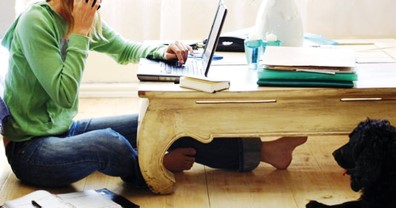
\includegraphics[scale=0.4]{images/smartwork.jpg}\\
  \vspace{12pt}

  \begin{itemize}
 	\item Growing (evolving) cities.
 \end{itemize}
 
 \vspace{12pt}

 \column{0.5\textwidth}
   \centering
    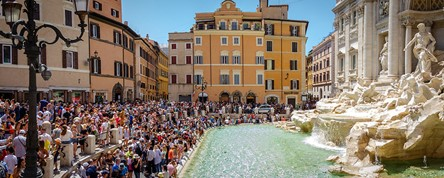
\includegraphics[scale=0.4]{images/overtourism.jpg}\\
    \vspace{12pt}
    
 	 \begin{itemize}
 		\item Changing habits
 	\end{itemize}
 	

	\vspace{12pt}

     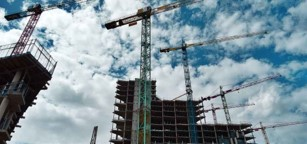
\includegraphics[scale=0.5]{images/growingtowns}\\
    \vspace{12pt}


   \end{columns}
  \end{frame}
  
  
  \begin{frame}{Waste Collection and Stochastic Elements}
  	\begin{columns}
  		\column{0.5\textwidth}
%  		\centering
		
   		\begin{itemize}
  			\item Unespected demand (during shifts)
  			\item Process (vehicles) disruption
  			\item Extra shifts
  			\item Need for new planning policies
  		\end{itemize}
  		
  		\vspace{12pt} 
  		
  		\column{0.5\textwidth}
  		\centering
  		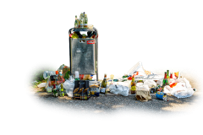
\includegraphics[scale=0.4]{images/waste.png}\\
  		\vspace{12pt}
  		
  		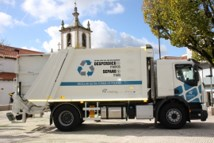
\includegraphics[scale=0.4]{images/truck.jpg}\\
		\vspace{12pt}
  				
  		
  		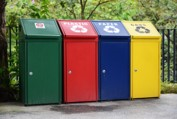
\includegraphics[scale=0.5]{images/bins.jpg}\\
  		\vspace{12pt}
  		
  		
  	\end{columns}
  \end{frame}
  
  \begin{frame}{The Problem addressed - vehicle routing problem with stochastic time-dependent demand increments}
  	
  	\begin{block}{}
  	
  	A homogeneous fleet of vehicles must visit a set of collection points with the aim of removing waste.
    \end{block}
    \begin{block}
  
  	We divide the planning horizon (day) in not-overlapping time slots.
    \end{block}
	\begin{block}
  	
  	Each collection point must be visited exactly once during the planning horizon and it has a known initial demand which may increase along the day.  The (uncertain) demand increments are revealed upon arrival at the collection points.
    \end{block}
    \begin{block}
  	
  	The goal is to minimize the expected total cost which also considers a penalty for the residual quantity of waste accumulated for the next day.
  \end{block}
  \end{frame}
  
    \begin{frame}{Stochastic Vehicle Routing}
  	\begin{block}{Routing with stochastic demand}
  	Waste collection routing problems with stochastic demand have been extensively	studied in the literature, mostly considering demand unknown but stationary. 
  	
  	Markov et al.\footnote{ I. Markov, M. Bierlaire, J.-F. Cordeau, Y. Maknoon, S. Varone, ``Waste collection inventory	routing with non-stationary stochastic demands'', Computers \& Operations Research 113, 104798 (2020)} deal with a demand varying on time. However, they consider a multi-period setting in which demands
  	may increase from one period to another, but it is constant over the same period (routes span over a single period, then the exact quantity is know at the beginning of the daily plan). 
  	
  	Conversely, we study a single day setting, where the time-horizon is
  	split in time-slots and routes can span over multiple time-slots. 
  	\end{block}
  \end{frame}
  

\begin{frame}{Problem Formulation}
Let $m$ be the number of available vehicles and $G$ a direct graph. Nodes $1,...,n$ of $G$ represent the collection points, whereas node $0$ and nodes $n+1,...,n+m$ represent the central depot (same location). 
\vspace{0.2cm}\\
Sets:
\begin{itemize}
	\item $V=\{0,1,...,n,n+1,...n+m\}:$ set of all nodes
	\item $V'=\{0,1,...,n\}=V\setminus\{n+1,...,n+m\}$ 
	\item $V''=\{1,...,n,n+1,...n+m\}=V\setminus\{0\}$ 
	\item $V'''=\{n+1,...n+m\}=V\setminus V'$ 
	\item $S:$ set of scenarios
	\item $T:$ set of periods
\end{itemize}
	
\end{frame}

\begin{frame}{The Problem - Parameters}
	%\resizebox{\textwidth}{!}{
 	%\begin{tabular}{ll}
	\begin{itemize}
		\item[]  $C$ \quad   vehicle capacity \\
		\item[] $c_{ij}$ \quad travel cost associated with arc $(i,j)$, $i\in V'$, $j\in V''$ ($j \neq i$) \\
		\item[] $t_{ij}$  \quad travel time associated with arc $(i,j)$, $i\in V'$, $j\in V''$ ($j \neq i$). \\
		%   \item $h_{i}:$ service time associated with node $i\in V'$, with $h_0=0$
		\item[] $e^t$  \quad starting time of period $t\in T$ \\
		\item[] $\ell^t$ \quad ending time of period $t\in T$ \\
		\item[] $p$  \quad unit penalty cost for uncollected waste\\
		\item[] $d_j$ \quad initial non-negative (deterministic) demand  $j=1,...,n$ \\
		\item[] $\delta_{jt}^s$  \quad non-negative demand increment $j=1,...,n$, (beginning) $t\in T$  $s \in S$ \\
		\item[] $M, T_{max}, Q_{max}$  \quad large constant \\
	\end{itemize}

	%\end{tabular}
	%}  

	\end{frame}



\begin{frame}{Formulation: Variables}
\begin{itemize}
	\item [$x_{ij}$]: binary variable equal to 1 if a vehicle travels from node $i \in V' $ to node $j \in V''$ ($j\neq i$), $0$ otherwise (first stage routes)
	\item [$U_{jt}$]: binary variable equal to 1 if node $j\in V''$ is visited in period $t \in T$
	\item [$\bar{T}_j$]: arrival time at node $j\in V$ 
	\item  [$y_{ij}^s$]: binary variable equal to 1 if a vehicle skips arc $(i,j)$ in scenario $s \in S$, $0$ otherwise 
	\item [$Q_j^s$]: theoretical cumulative load at node $j\in V$ in scenario $s \in S$
	\item [$R_j^s$]: quantity of waste exceeding the capacity at node $j=n+1,...,n+m$ in scenario $s \in S$
	\item [$L_j^s$]: quantity of waste accumulated at collection point $j=1,...,n$ in scenario $s \in S$ in periods following its visit, and left over for the next day
	\item [$\rho_j^s$]: binary variable equal to 1 if node $j=1,...,n$ is associated with  event ``capacity saturation'' in scenario $s\in S$, $0$ otherwise 
	\item [$\alpha_j^s$]: binary variable equal to 1 if node $j$ is the first node associated with  event ``capacity saturation'' in scenario $s\in S$, $0$ otherwise
\end{itemize}
	
\end{frame}

	\begin{frame}{Example}
	\begin{figure}
		\centering
		\scalebox{0.8}{
			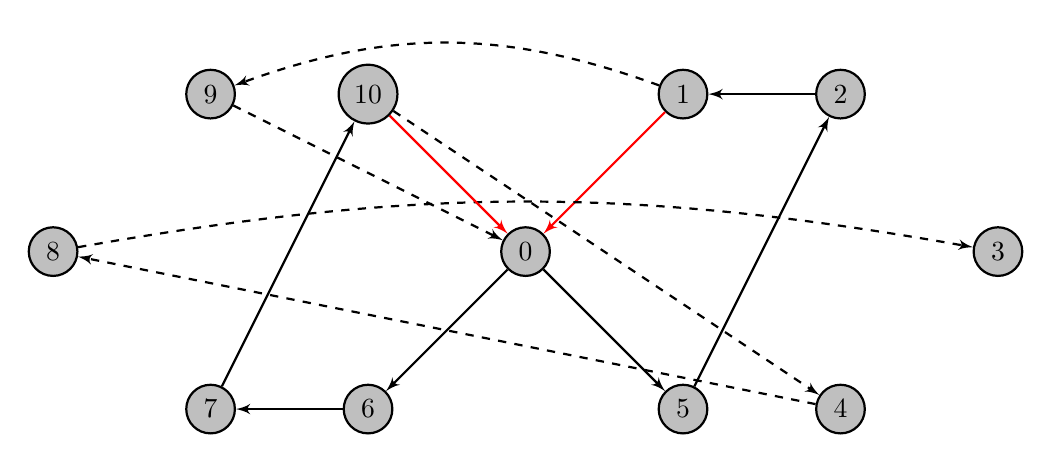
\begin{tikzpicture}
				\tikzset{
					edge/.style = {->,> = latex', thick},
					vertex/.style = {shape=circle,draw, fill=lightgray, thick}  % size of the circle diameter
				}
				\node[vertex] (n0) at  (0,0){0};
				\node[vertex] (n1) at  (2, 2){1};
				\node[vertex] (n2) at  (4, 2){2};
				\node[vertex] (n3) at  (6, 0){3};
				\node[vertex] (n4) at  (4, -2){4};
				\node[vertex] (n5) at  (2, -2){5};
				\node[vertex] (n6) at  (-2, -2){6};
				\node[vertex] (n7) at  (-4, -2){7};
				\node[vertex] (n8) at  (-6, 0){8};
				\node[vertex] (n9) at  (-4, 2){9};
				\node[vertex] (n10) at  (-2, 2){10};
				
				\draw[edge] (n0) to node{} (n5);
				\draw[edge] (n5) to node{} (n2);
				\draw[edge] (n2) to node{} (n1);
				\draw[edge, in=20, out=160, dashed] (n1) to node{} (n9);
				\draw[edge,dashed] (n9) to node{} (n0);
				\draw[edge, red] (n1) to node{} (n0);
				\draw[edge] (n0) to node{} (n6);
				\draw[edge] (n6) to node{} (n7);
				\draw[edge] (n7) to node{} (n10);
				\draw[edge, dashed] (n10) to node{} (n4);
				\draw[edge, dashed] (n4) to node{} (n8);
				\draw[edge, out=10, in=170, dashed] (n8) to node{} (n3);
				\draw[edge, red] (n10) to node{} (n0);
			\end{tikzpicture}
		}
		\caption{ Dashed arcs ($- \rightarrow$) consider $y_{i,j}^s=1$ and $x_{ij}=1$, continuous arcs ($\longrightarrow$) consider $y_{i,j}^s=0$ and $x_{ij}=1$, while red arcs ({\color{red}$\longrightarrow$}) are the arcs connecting the vehicles to the depot ($\alpha_j^s=1$).}
		\label{fig:solution}
	\end{figure}
\end{frame}

	\begin{frame}{Formulation: Objective Function}
		\begin{block}{}
			$$
			\min \quad  \sum_{i \in V'} \sum_{j \in V'' (j\neq i)} c_{ij} {x}_{ij} - \frac{1}{|S|} \sum_{s \in S} \sum_{i=1}^n \sum_{j \in V''(j\neq i)} c_{ij} {y}_{ij}^s + \frac{1}{|S|} \sum_{s \in S} \sum_{j=1}^n  c_{j0} \alpha_j^s + 
			$$
			\begin{equation}\label{of}
				+ \frac{1}{|S|} \sum_{s \in S} \sum_{j=n+1}^{n+m}  p R_j^s + \frac{1}{|S|} \sum_{s \in S} \sum_{j=1}^n p L_j^s
			\end{equation}
			
		\end{block}
		
		$$\min Z = Z_1 - Z_2 + Z_3 + Z_4 + Z_5$$
		
	\end{frame} 


	\begin{frame}{Formulation: Constraints (1/4)}
	
	\begin{block}{}
		\begin{equation}\label{c1}
			\sum_{j \in V''\setminus\{i\}} x_{ij} = \sum_{j \in V'\setminus\{i\}}x_{ji} = \sum_{t\in T}U_{it}, \quad i=1,...,n 
		\end{equation}

		\begin{equation}\label{c2}
			\sum_{j \in V''}x_{0j} = m 
		\end{equation}

		\begin{equation}\label{c3}
			\sum_{j \in V'} x_{ji} = 1, \quad i=n+1,...,n+m 
		\end{equation}
	
		\begin{equation}\label{c4}
			\sum_{t\in T}U_{jt}=1, \quad j\in V''
		\end{equation}
	
		\begin{equation}\label{c5}
			\bar{T}_0=0 
		\end{equation}
		
		\begin{equation}\label{c5'}
			\bar{T}_j \geq \bar{T}_i + t_{ij}-M(1-x_{ij}), \quad \ i \in V', j \in V''(j \neq i)
		\end{equation}
	\end{block}
	
	\end{frame}


	\begin{frame}{Formulation: Constraints (2/4)}
	
	\begin{block}{}
		\begin{equation}\label{c6}
			e^t - T_{max} (1-U_{jt}) \leq \bar{T}_j \leq \ell^t + T_{max} (1-U_{jt}), \quad j \in V'', t \in T
		\end{equation}
		
		\begin{equation}\label{c7}
			Q_0^s =0, \quad  s \in S
		\end{equation}
		
		\begin{equation}\label{c8}
			Q_j^s \geq Q_i^s -M(1-x_{ij})+ d_j +\sum_{t\in T}\sum_{\tau=1}^t\delta_{j\tau}^sU_{jt}, \quad s \in S, i\in V', j=1,...,n  
		\end{equation}
		
		\begin{equation}\label{c8.1}
			Q_j^s \leq Q_i^s + M(1-x_{ij})+ d_j +\sum_{t\in T}\sum_{\tau=1}^t\delta_{j\tau}^sU_{jt}, \quad s \in S, i\in V', j=1,...,n   
		\end{equation}

	\end{block}
	\end{frame}


	

\begin{frame}{Formulation: Constraints (3/4)}
	\begin{block}{}
		\begin{equation}\label{c9}
			Q_i^s -M(1-x_{ij}) \leq	Q_j^s \leq Q_i^s + M(1-x_{ij}), \quad s \in S, i\in V''' 
		\end{equation}
		
		\begin{equation}\label{c10}
			R_j^s\geq Q_j^s - C , \quad s \in S, j=n+1,...,n+m 
		\end{equation}
		
		\begin{equation}\label{c11}
			R_j^s\geq 0, \quad s \in S, j=n+1,...,n+m 
		\end{equation}
		
		\begin{equation}\label{c12}
			L_j^s=\sum_{t\in T}\sum_{\tau=t+1}^{|T|}\delta_{j\tau}^sU_{jt}, \quad s \in S, j=1,...,n 
		\end{equation}

	\end{block}
\end{frame}

\begin{frame}{Formulation: Constraints (4/4)}
	\begin{block}{}
			
			\begin{equation}\label{c14}
			\frac{Q_j^s-C}{Q_{max}}	\leq \rho_j^s \leq 1-\frac{C-Q_j^s}{Q_{max}}, \quad s \in S, j = 1, \ldots ,n 
			\end{equation}
			
			\begin{equation}\label{c15}
				y_{ij}^s \leq \frac{1}{2}(x_{ij}+\rho_i^s), \quad s \in 	S, i=1,...,n, j \in V'' (j \neq i)
			\end{equation}
		
			\begin{equation} \label{cy}
				y_{0j}^s = 0, \quad s \in S, \quad j \in V''
			\end{equation}
		
		\begin{equation} \label{cyalpha}
			\alpha_j^s = \sum_{i \in V''}y_{ji}^s - \sum_{i \in V'}y_{ij}^s, \quad s \in S, \quad j = 1, \ldots, n
		\end{equation}
	\end{block}
\end{frame}

\begin{frame}{Realistic Instance - Different types of customers}
	\begin{table}[]
		\centering
		%\caption{}
		\label{tab:realinstance}
		\scalebox{0.7}{
		\begin{tabular}{l|l|llll}
			\hline
			 user type & demand ($d_j$)   & \multicolumn{4}{c}{delta ($\delta_{jt}^s$) and timeslot [$e^t$, $l^t$]}              \\
			\hline
			&          & [8:00, 12:00]     & [12:00, 16:00]  & [16.00, 20:20]     & [20:00, 24:00]:  \\
			\hline
			home       & medium   & medium   & low    & low       & medium \\
			school     & very low & low      & medium & high      & low    \\
			restaurant & high     & very low & medium & very high & medium \\
			
			bar        & low      & high     & high   & high      & high \\
			\hline 
		\end{tabular}
		}
	\end{table}
\end{frame}


\begin{frame}{Realistic Instance}
	\begin{center}
		\includegraphics[scale=0.35]{images/real\_instance.jpg}
	\end{center}
\end{frame}

\begin{frame}{Realistic Instance: results and comments}
	
	\begin{table}[]
		\centering
		\caption{results realistic instance}
		\label{tab:resreal}
		\scalebox{0.8}{
			\begin{tabular}{lll}
				\hline
				Inst name      & I1\_R2        & I1\_R2\_EEV \\
				\hline
				objValue       & 9496.31       & 10070.03    \\
				Z1             & 12607.92      & 11657.46    \\
				Z2             & 9677.65       & 5875.45     \\
				Z3             & 570.04        & 1444.02     \\
				Z4             & 3540.00       & 1794.00     \\
				Z5             & 2456.00       & 1050.00     \\
				\hline
				\multicolumn{2}{l}{Difference} & 6.04\%  \\
				\hline    
			\end{tabular}
		}
	\end{table}
	\begin{itemize}
		
		\item different path / end of shift stratgy
	\end{itemize}
\end{frame}


\begin{frame}{Computational Experiments: Instances}
	\begin{table}[]
		\centering
		\caption{Instances parameters}
		\label{tab:instances}
		\scalebox{0.7}{
		    \begin{tabular}{cc}
				\hline
				Parameter & Value \\
				\hline
				$n$     & [5,7,10] \\
				$m$     &	3 \\
				Depot	& [Central, Located lower left] \\
				%$C$	    & [100, 150, 200] \\
				$|T|$	&  3  \\
				$|S|$   &	5 \\
				$Tmax$  &	[30, 50, 100] \\
				Average $D$     &	50 \\
				Average $\delta$ &	10 \\
				\hline
			\end{tabular}
		}
	\end{table}
	\begin{block}{Patterns for customers}
		\begin{itemize}
			\item \textit{type 1}: $d$ low; $\delta$ high, low, low
			\item \textit{type 2}: $d$ medium; $\delta$ medium, high, low
			\item \textit{type 3}: $d$ high; $\delta$ low, low, medium.
		\end{itemize}
	\end{block}
\end{frame}

\begin{frame}{Computational Experiments: Results}
	\begin{table}[]
		\centering
		\caption{Results 5, 7 customers}
		\label{tab:my-table5-7a}
		\scalebox{0.7}{
	\begin{tabular}{llllll}
		\hline
		\textbf{name} & \textbf{objVal} & \textbf{EVVobjVal} &\textbf{Delta} & \textbf{runTime} &\textbf{gap} \\
		\hline
		I2\_N5\_T30\_C100\_0 & 1840.29  & 1845.71  & 0.29    & 2.16       & 0.00      \\
		I2\_N5\_T30\_C150\_0   & 648.80   & 657.08  & 1.28   & 2.30   & 0.00 \\
		I2\_N5\_T30\_C200\_0 & 23.71 & 25.77 & 8.69    & 0.86& 0.00 \\
		\hline
		I2\_N5\_T100\_C100\_0& 1840.29    & 1845.04    & 0.26  & 2.49     & 0.00 \\
		I2\_N5\_T100\_C150\_0 & 648.80    & 657.08     & 1.28  & 1.78  & 0.00 \\
		I2\_N5\_T100\_C200\_0& 23.71  & 25.77 & 8.69 & 0.65 & 0.00  \\
		\hline
		I2\_N7\_T30\_C100\_0 & 1474.07 & 1486.94 & 0.87 & 260.92 & 0.00 \\
		I2\_N7\_T30\_C120\_0 & 881.51  & 889.51  & 0.91 & 274.45 & 0.00 \\
		I2\_N7\_T30\_C140\_0& 309.43  & 323.27  & 4.47  & 218.17 & 0.00  \\
		I2\_N7\_T30\_C210\_0  & 26.53  & 26.53  & 0.00  & 1.29 & 0.00 \\
		%I2\_N7\_T30\_C280\_0  & 26.30  & 26.30   & 0.00   & 1.41 & 0.00\\
		\hline
		I2\_N7\_T100\_C100\_0 & 1474.07 & 1486.94 & 0.87 & 280.01 & 0.00 \\
		I2\_N7\_T100\_C120\_0 & 879.69  & 889.51  & 1.12 & 272.15 & 0.00 \\
		I2\_N7\_T100\_C140\_0 & 307.62 & 323.27& 5.09  & 197.23  & 0.00  \\
		I2\_N7\_T100\_C210\_0 & 26.36 & 26.36 & 0.00  & 5.72   & 0.00 \\
		%I2\_N7\_T100\_C280\_0& 24.99  & 24.99 & 0.00 & 6.98  & 0.00 \\
		\hline                           
	\end{tabular}
		}
	\end{table}
\end{frame}

\begin{frame}{Computational Experiments: Results}
	\begin{table}[]
		\centering
		\caption{Results 5, 7 customers}
		\label{tab:my-table5-7b}
		\scalebox{0.6}{
	\begin{tabular}{lrrrrrrrrrr}
		\hline
		\textbf{name}                  & \textbf{Z1}    & \textbf{Z2}   & \textbf{Z3}   & \textbf{Z4}      & \textbf{Z5}     & \textbf{Z1EVV} & \textbf{Z2EVV} & \textbf{Z3EVV} & \textbf{Z4EVV}   & \textbf{Z5EVV} \\
		\hline
		I2\_N5\_T30\_C100\_0  & 25.46 & 9.25 & 2.95 & 1664.05 & 157.08 & 22.03 & 7.46  & 3.84  & 1381.34 & 445.95  \\
		I2\_N5\_T30\_C150\_0  & 23.71 & 0.00 & 0.00 & 625.09  & 0.00   & 22.78 & 0.00  & 0.00  & 199.44  & 434.86  \\
		I2\_N5\_T30\_C200\_0  & 23.71 & 0.00 & 0.00 & 0.00    & 0.00   & 21.53 & 0.00  & 0.00  & 4.24    & 0.00    \\
		\hline
		I2\_N5\_T100\_C100\_0 & 25.46 & 9.08 & 2.79 & 1821.13 & 0.00   & 22.03 & 8.97  & 4.69  & 1423.58 & 403.71  \\
		I2\_N5\_T100\_C150\_0 & 23.71 & 0.00 & 0.00 & 625.09  & 0.00   & 22.78 & 0.00  & 0.00  & 199.44  & 434.86  \\
		I2\_N5\_T100\_C200\_0 & 23.71 & 0.00 & 0.00 & 0.00    & 0.00   & 21.53 & 0.00  & 0.00  & 4.24    & 0.00    \\
		\hline
		I2\_N7\_T30\_C100\_0  & 29.63 & 14.44 & 3.98 & 1394.52 & 60.37 & 35.26 & 19.38 & 2.50 & 1304.92 & 163.64 \\
		I2\_N7\_T30\_C120\_0  & 27.53 & 1.86  & 0.95 & 801.81  & 53.08 & 27.41 & 8.39  & 3.96 & 610.40  & 256.13 \\
		I2\_N7\_T30\_C140\_0  & 33.86 & 0.00 & 0.00 & 225.26  & 50.31  & 31.34 & 1.43  & 1.43  & 291.93  & 0.00    \\
		I2\_N7\_T30\_C210\_0  & 26.53 & 0.00 & 0.00 & 0.00    & 0.00   & 26.53 & 0.00  & 0.00  & 0.00    & 0.00    \\

		%I2\_N7\_T30\_C280\_0  & 26.30 & 0.00 & 0.00 & 0.00    & 0.00   & 26.30 & 0.00  & 0.00  & 0.00    & 0.00    \\
		\hline
		I2\_N7\_T100\_C100\_0 & 29.63 & 13.67 & 3.22 & 1454.89 & 0.00 & 32.18 & 17.88 & 4.08 & 1246.41 & 222.15 \\
		I2\_N7\_T100\_C120\_0 & 27.53 & 6.34  & 3.61 & 854.89  & 0.00 & 30.39 & 7.53  & 0.12 & 610.40  & 256.13 \\
		I2\_N7\_T100\_C140\_0 & 32.05 & 0.00 & 0.00 & 275.57  & 0.00   & 31.34 & 0.00  & 0.00  & 291.93  & 0.00    \\
		I2\_N7\_T100\_C210\_0 & 26.36 & 0.00 & 0.00 & 0.00    & 0.00   & 26.36 & 0.00  & 0.00  & 0.00    & 0.00    \\
		%I2\_N7\_T100\_C280\_0 & 24.99 & 0.00 & 0.00 & 0.00    & 0.00   & 24.99 & 0.00  & 0.00  & 0.00    & 0.00  \\
		\hline 
	\end{tabular}
		}
	\end{table}
\end{frame}

\begin{frame}{computational Experiments: results}
	\begin{figure}
		\centering
			\includegraphics[scale=0.5]{images/gap5Customers.png}
			\caption{5 customers}
	\end{figure}

\end{frame}

\begin{frame}{Computational Experiments: Results}
	\begin{table}[]
		\centering
		\caption{Results 10 customers}
		\label{tab:my-tableN10a}
		\scalebox{0.7}{
			\begin{tabular}{lrrrrr}
				\hline
				\textbf{name} & \textbf{objVal} & \textbf{EVVobjVal} &\textbf{Delta} & \textbf{runTime} &\textbf{gap} \\
				\hline
				I2\_N10\_T30\_C275\_0  & 91.15 & 140.48 & 54.12  & 555.26  & 0.00 \\
				I2\_N10\_T30\_C300\_0  & 34.73 & 44.94  & 29.39  & 24.55   & 0.00 \\
				I2\_N10\_T30\_C325\_0  & 33.07 & 33.07  & 0.00   & 15.14   & 0.00 \\
				I2\_N10\_T30\_C350\_0  & 30.17 & 30.20  & 0.10   & 21.38   & 0.00 \\
				I2\_N10\_T30\_C400\_0  & 30.17 & 30.17  & 0.00   & 7.19    & 0.00 \\
				\hline
				I2\_N10\_T100\_C275\_0 & 47.70 & 56.63  & 18.73  & 1109.94 & 0.00 \\
				I2\_N10\_T100\_C300\_0 & 34.73 & 153.02 & 340.60 & 248.36  & 0.00 \\
				I2\_N10\_T100\_C325\_0 & 33.07 & 33.07  & 0.00   & 347.44  & 0.00 \\
				I2\_N10\_T100\_C350\_0 & 30.17 & 30.20  & 0.10   & 198.87  & 0.00 \\
				I2\_N10\_T100\_C400\_0 & 30.17 & 30.17  & 0.00   & 180.40  & 0.00 \\
				\hline                           
			\end{tabular}
		}
	\end{table}
\end{frame}




\begin{frame}{Computational Experiments: Results 10 customers}
	\begin{table}[]
		\centering
		\caption{Results}
		\label{tab:my-tableN10b}
		\scalebox{0.6}{
			\begin{tabular}{lrrrrrrrrrr}
				\hline
				\textbf{name}                  & \textbf{Z1}    & \textbf{Z2}   & \textbf{Z3}   & \textbf{Z4}      & \textbf{Z5}     & \textbf{Z1EVV} & \textbf{Z2EVV} & \textbf{Z3EVV} & \textbf{Z4EVV}   & \textbf{Z5EVV} \\
				\hline
				I2\_N10\_T30\_C275\_0  & 40.21 & 0.00 & 0.00 & 9.36 & 41.58 & 42.84 & 1.39 & 1.39 & 97.64 & 0.00   \\
				I2\_N10\_T30\_C300\_0  & 34.73 & 0.00 & 0.00 & 0.00 & 0.00  & 33.22 & 0.00 & 0.00 & 11.72 & 0.00   \\
				I2\_N10\_T30\_C325\_0  & 33.07 & 0.00 & 0.00 & 0.00 & 0.00  & 33.07 & 0.00 & 0.00 & 0.00  & 0.00   \\
				I2\_N10\_T30\_C350\_0  & 30.17 & 0.00 & 0.00 & 0.00 & 0.00  & 30.17 & 0.00 & 0.00 & 0.03  & 0.00   \\
				I2\_N10\_T30\_C400\_0  & 30.17 & 0.00 & 0.00 & 0.00 & 0.00  & 30.17 & 0.00 & 0.00 & 0.00  & 0.00   \\
				\hline
				I2\_N10\_T100\_C275\_0 & 42.65 & 0.00 & 0.00 & 5.05 & 0.00  & 38.17 & 0.00 & 0.00 & 18.46 & 0.00   \\
				I2\_N10\_T100\_C300\_0 & \textbf{34.73} & 0.00 & 0.00 & 0.00 & 0.00  & \textbf{33.22} & 0.00 & 0.00 & 0.00  & \textbf{119.80} \\
				I2\_N10\_T100\_C325\_0 & 33.07 & 0.00 & 0.00 & 0.00 & 0.00  & 33.07 & 0.00 & 0.00 & 0.00  & 0.00   \\
				I2\_N10\_T100\_C350\_0 & 30.17 & 0.00 & 0.00 & 0.00 & 0.00  & 30.17 & 0.00 & 0.00 & 0.03  & 0.00   \\
				I2\_N10\_T100\_C400\_0 & 30.17 & 0.00 & 0.00 & 0.00 & 0.00  & 30.17 & 0.00 & 0.00 & 0.00  & 0.00\\
				\hline 
			\end{tabular}
		}
	\end{table}
	%genarally speaking, EEV has a 0\% gap from the stochastic in the situations in which it is sure or that at the end of the proceess some waste will be left or at the opposite if it is sure that in each scenario all waste will be collected.
\end{frame}

\begin{frame}{Solution comments}
	
\begin{columns}
	\column{0.4\textwidth}
	Instance S\_6
	\begin{itemize}
		\item Stochastic
		\begin{itemize}
			\item $0 \rightarrow 1 \rightarrow 7 \rightarrow 10 \rightarrow 4 \rightarrow  12$
			\item $0 \rightarrow 2 \rightarrow 3 \rightarrow 6 \rightarrow 11$
			\item $0 \rightarrow 8 \rightarrow 9 \rightarrow 5 \rightarrow 13$
		\end{itemize}
		\item EEV
		\begin{itemize}
			\item $0 \rightarrow 1 \rightarrow 7 \rightarrow 10 \rightarrow 9 \rightarrow  11$
			\item $0 \rightarrow {\color{blue}5} \rightarrow 2 \rightarrow 3 \rightarrow 6 \rightarrow 13$
			\item $0 \rightarrow 8 \rightarrow 4 \rightarrow 12$
		\end{itemize}
	\end{itemize}
	
	\column{0.6\textwidth}
	\centering
	\includegraphics[scale=0.3]{images/plot\_S6\_stochastic.png}\\

	
	\includegraphics[scale=0.3]{images/plot\_S6\_fix.png}\\

	
	\end{columns}
	%Customer 5 could be skipped by EEV if route blue would be traveled in the opposite order.
	
\end{frame}

\begin{frame}{Policies}
	\begin{itemize}
		\item \textbf{P1:} solve a standard VRP with demand equal to the initial demand (completely neglecting future demand $\delta_{jt}^s$)
		
		\item \textbf{P2:} solve a standard VRP with demand equal to the initial demand + expected value of the sum of the additional demands delta ($\delta_{jt}^s$). More conservative policy 
		
		\item \textbf{P3:} solve a standard VRP with demand equal to the initial demand + expected value of the sum of the additional demands up to the central time slot. Less  conservative than P2.
		
	\end{itemize}
		
\end{frame}

\begin{frame}{Policies}
	\begin{itemize}
		
		\item \textbf{P4:} P2 + with vehicle capacity reduced by x\% $\rightarrow$ 10\% (cushion to be used for unexpected extra demand)
		
		\item \textbf{P5:} P2 + half of the vehicle have increased capacity and the other half have reduced capacity by x\% $\rightarrow$ 15\%
		
		\item \textbf{P6:} P2 + modified objective function  (the goal is to insert the farthest nodes at the end of the routes, so in case of skipping we skip the longest arcs). $\min \left[ \sum_{j \in V''} \frac{1}{d_{0j}} \cdot u_{j} + K\sum_{j \in V} \mu_j \right]$.
	\end{itemize}
\end{frame}

\begin{frame}{Computational Experiments: Policies Results 5 customers}
	\begin{table}[]
		\centering
		\caption{Results policies 5 customers}
		\label{tab:policiesN5}
		\scalebox{0.6}{
		\begin{tabular}{lrrrrrrr}
			\hline
				\textbf{name}  & \textbf{objVal}  & \textbf{delta}   & \textbf{Z1}    & \textbf{Z2}    & \textbf{Z3}   & \textbf{Z4}      & \textbf{Z5}     \\
				\hline
				I2\_N5\_T30\_C100\_0     & 1840.29 & 0.00  & 25.46 & 9.25  & 2.95 & 1664.05 & 157.08 \\
				I2\_N5\_T30\_C100\_0\_P1 & 1842.52 & 0.00  & 23.71 & 7.25  & 4.93 & 1196.58 & 624.55 \\
				I2\_N5\_T30\_C100\_0\_P2 & 1848.66 & 0.00  & 22.03 & 5.85  & 5.19 & 1580.66 & 246.63 \\
				I2\_N5\_T30\_C100\_0\_P3 & 1842.24 & 0.00  & 22.78 & 4.86  & 3.20 & 1357.84 & 463.29 \\
				I2\_N5\_T30\_C100\_0\_P4 & 1878.35 & 0.02  & 21.53 & 5.77  & 5.77 & 1142.72 & 714.10 \\
				I2\_N5\_T30\_C100\_0\_P5 & 1878.35 & 0.02  & 21.53 & 5.77  & 5.77 & 1142.72 & 714.10 \\
				I2\_N5\_T30\_C100\_0\_P6 & 1875.17 & 0.02  & 23.99 & 11.35 & 5.72 & 1515.02 & 341.80 \\
				\hline
				I2\_N5\_T30\_C150\_0     & 648.80  & 0.00  & 23.71 & 0.00  & 0.00 & 625.09  & 0.00   \\
				I2\_N5\_T30\_C150\_0\_P1 & 964.38  & 0.49  & 19.89 & 0.00  & 0.00 & 737.82  & 206.67 \\
				I2\_N5\_T30\_C150\_0\_P2 & 657.08  & 0.01  & 22.78 & 0.00  & 0.00 & 199.44  & 434.86 \\
				I2\_N5\_T30\_C150\_0\_P3 & 650.55  & 0.00  & 25.46 & 0.71  & 0.71 & 350.31  & 274.78 \\
				I2\_N5\_T30\_C150\_0\_P4 & 657.08  & 0.01  & 22.78 & 0.42  & 0.42 & 199.44  & 434.86 \\
				I2\_N5\_T30\_C150\_0\_P5 & 650.55  & 0.00  & 25.46 & 0.00  & 0.00 & 281.94  & 343.15 \\
				I2\_N5\_T30\_C150\_0\_P6 & 875.11  & 0.35  & 23.99 & 0.71  & 0.71 & 281.13  & 569.99 \\
				\hline
				I2\_N5\_T30\_C200\_0     & 23.71   & 0.00  & 23.71 & 0.00  & 0.00 & 0.00    & 0.00   \\
				I2\_N5\_T30\_C200\_0\_P1 & 870.08  & 35.70 & 18.40 & 6.68  & 3.78 & 795.00  & 59.58  \\
				I2\_N5\_T30\_C200\_0\_P2 & 25.77   & 0.09  & 21.53 & 0.00  & 0.00 & 4.24    & 0.00   \\
				I2\_N5\_T30\_C200\_0\_P3 & 60.22   & 1.54  & 19.89 & 0.00  & 0.00 & 40.33   & 0.00   \\
				I2\_N5\_T30\_C200\_0\_P4 & 25.46   & 0.07  & 25.46 & 0.00  & 0.00 & 0.00    & 0.00   \\
				I2\_N5\_T30\_C200\_0\_P5 & 60.22   & 1.54  & 19.89 & 0.00  & 0.00 & 40.33   & 0.00   \\
				I2\_N5\_T30\_C200\_0\_P6 & 119.43  & 4.04  & 23.99 & 0.00  & 0.00 & 95.44   & 0.00  \\  
				\hline 
			\end{tabular}
		}
	\end{table}
\end{frame}

\begin{frame}{Computational Experiments: Policies Results 10 customers}
	\begin{table}[]
		\centering
		\label{tab:policiesN10}
		\scalebox{0.5}{
			\begin{tabular}{lrrrrrrr}
				\hline
				\textbf{name}  & \textbf{objVal}  & \textbf{delta}   & \textbf{Z1}    & \textbf{Z2}    & \textbf{Z3}   & \textbf{Z4}      & \textbf{Z5}     \\
				\hline
				I2\_N10\_T30\_C275\_0     & 91.15   & 0.00  & 40.21 & 0.00 & 0.00 & 9.36    & 41.58  \\
				I2\_N10\_T30\_C275\_0\_P1 & 973.50  & 9.68  & 30.17 & 8.43 & 7.97 & 661.31  & 282.47 \\
				I2\_N10\_T30\_C275\_0\_P2 & 104.43  & 0.15  & 38.17 & 0.62 & 0.62 & 6.17    & 60.09  \\
				I2\_N10\_T30\_C275\_0\_P3 & 976.19  & 9.71  & 32.41 & 4.00 & 4.00 & 432.87  & 510.91 \\
				I2\_N10\_T30\_C275\_0\_P4 & 105.30  & 0.16  & 39.04 & 0.62 & 0.62 & 6.17    & 60.09  \\
				I2\_N10\_T30\_C275\_0\_P5 & 551.11  & 5.05  & 44.86 & 0.00 & 0.00 & 207.15  & 299.10 \\
				I2\_N10\_T30\_C275\_0\_P6 & 773.47  & 7.49  & 45.78 & 5.34 & 5.34 & 154.40  & 573.29 \\
				\hline
				I2\_N10\_T30\_C325\_0     & 33.07   & 0.00  & 33.07 & 0.00 & 0.00 & 0.00    & 0.00   \\
				I2\_N10\_T30\_C325\_0\_P1 & 1396.78 & 41.24 & 29.23 & 6.05 & 6.05 & 1153.10 & 214.46 \\
				I2\_N10\_T30\_C325\_0\_P2 & 94.44   & 1.86  & 33.07 & 0.00 & 0.00 & 0.00    & 61.37  \\
				I2\_N10\_T30\_C325\_0\_P3 & 257.05  & 6.77  & 30.17 & 1.64 & 1.64 & 58.79   & 168.09 \\
				I2\_N10\_T30\_C325\_0\_P4 & 33.22   & 0.00  & 33.22 & 0.00 & 0.00 & 0.00    & 0.00   \\
				I2\_N10\_T30\_C325\_0\_P5 & 181.96  & 4.50  & 32.48 & 0.52 & 0.52 & 149.48  & 0.00   \\
				I2\_N10\_T30\_C325\_0\_P6 & 441.41  & 12.35 & 45.78 & 0.00 & 0.00 & 0.00    & 395.63 \\
				\hline
				I2\_N10\_T30\_C350\_0     & 30.17   & 0.00  & 30.17 & 0.00 & 0.00 & 0.00    & 0.00   \\
				I2\_N10\_T30\_C350\_0\_P1 & 918.64  & 29.45 & 29.23 & 5.07 & 5.07 & 720.30  & 169.11 \\
				I2\_N10\_T30\_C350\_0\_P2 & 30.20   & 0.00  & 30.17 & 0.00 & 0.00 & 0.03    & 0.00   \\
				I2\_N10\_T30\_C350\_0\_P3 & 934.62  & 29.98 & 29.23 & 2.58 & 2.58 & 642.71  & 262.68 \\
				I2\_N10\_T30\_C350\_0\_P4 & 33.07   & 0.10  & 33.07 & 0.00 & 0.00 & 0.00    & 0.00   \\
				I2\_N10\_T30\_C350\_0\_P5 & 239.26  & 6.93  & 30.90 & 1.41 & 1.41 & 32.61   & 175.75 \\
				I2\_N10\_T30\_C350\_0\_P6 & 441.41  & 13.63 & 45.78 & 0.00 & 0.00 & 0.00    & 395.63 \\
				\hline 
			\end{tabular}
		}
	\end{table}
\end{frame}




\begin{frame}{Conclusion}
	\begin{itemize}
		\item waste collection / waste management important for urban grow and sustainability
		\item cities evolves, dynamics and uncertainty to manage in order to offer proper services
		\item New stochastic model for waste collection
		\item Difficult to solve $\rightarrowtail$ policies are easier in general.
	\begin{itemize}
		\item  lower capacity for vehicles
		\item try to serve farthest users as last (fair?)
		\item late collection
		\item robust plan 
	\end{itemize}
	\end{itemize}
	\vspace{20pt}

	
\end{frame}

\begin{frame}{Conclusion}
\begin{center}
	\textbf{Thank You!}\\
	\vspace{15pt}
	Giuseppe Stecca\\
	giuseppe.stecca@iasi.cnr.it\\
	\vspace{20pt}
	
\includegraphics[width=2.5cm]{images/iasicnr} \\
	\vspace{10pt}

\end{center}
\end{frame}
\end{document}

